%mac
%\loai{Tính moment lực khi đã biết lực và cánh tay đòn}

%\loai{Tính moment lực khi chưa biết cánh tay đòn}
\begin{vidu}%[1P2C9.2K][Loai1]
Một cái thước dài $ \ell=1\ m $ thẳng, đồng chất, tiết diện đều có thể quay quanh một trục nằm ngang đi qua một đầu của thước. Cho khối lượng của thước là $ m=800\ g $. Lấy $ g=10\ m/s^2 $. Hãy tính moment của trọng lực đối với trục quay khi thước hợp với phương thẳng đứng một góc: $ 0^\circ$; $ 30^\circ $; $ 45^\circ$; $60^\circ$.
\haidong{15}
\loigiai{
\immini{Gọi $ \alpha $ là góc hợp bởi thước với phương thẳng đứng.
\begin{itemize}
\item Do thước thẳng đồng chất, tiết diện đều nên trọng lực có điểm đặt ở chính giữa thước.
\item Cánh tay đòn của trọng lực đối với trục quay O: $ d=\dfrac{\ell}{2}.\sin \alpha $ 
\item Moment của trọng lực đối với trục quay O: 
\begin{align*}
M=P.d=mg.\dfrac{\ell}{2}.\sin \alpha=0,8.10.\dfrac 1 2.\sin \alpha=4.\sin \alpha
\end{align*} 
\begin{itemize}
\item $ \alpha=0^\circ \Rightarrow M=4.\sin 0^\circ=0\ N.m $ 
\item $ \alpha=30^\circ \Rightarrow M=4.\sin 30^\circ=2\ N.m $ 
\item $ \alpha=45^\circ \Rightarrow M=4.\sin 45^\circ=2\sqrt 2\ N.m $ 
\item $ \alpha=60^\circ \Rightarrow M=4.\sin 60^\circ=2\sqrt 3\ N.m $
\end{itemize}	
\end{itemize}}{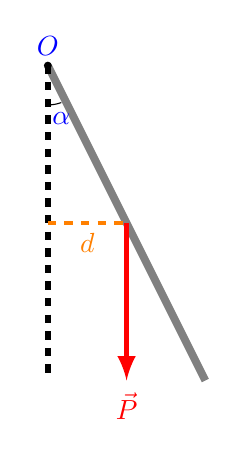
\begin{tikzpicture}
\draw  [line  width=0.1cm,gray]  (-1,2)  --  (1,-2);
\draw  [dashed,line  width=2]  (-1,2)  --  (-1,-2);
\draw  [-latex,line  width=2,red]  (0,0)  --  (0,-2) node[below]{\normalsize{$\vec{P}$}};
\draw  [dashed,line  width=1.5,orange]  (-1,0)  --  (0,0);
\node at (-.5,0)  [below,orange]  {$  d  $};
\draw  (-1,1.5)  arc  [radius=0.5cm,  start  angle=270,  end  angle=  290]node[below,blue]{\normalsize{$\alpha$}};
\fill  (-1,2)  circle  (.05)  node  [above,blue]  {$O$};

\end{tikzpicture}}}
\end{vidu}
\begin{vidu}%[1P2C9.2K][Loai1] 
\immini[thm]{Thanh nhẹ $OB$ có thể quay quanh $O$. Tác dụng lên thanh các lực $\vec{F}_1$ và $\vec{F}_2$ đặt tại $A$ và $B$ như hình. Biết $F_1 = 20\ N$, $OA = 10\ cm$, $AB = 40\ cm$. Thanh cân bằng, $\vec{F}_1$ và $\vec{F}_2$ hợp với $AB$ các góc $\alpha$ , $\beta$. Tìm $F_2$ nếu:
\begin{itemize}
\item[a.]$\alpha  = \beta  = 90^\circ$ 
\item[b.]$\alpha  = 30^\circ $, $\beta  = 90^\circ$ 
\item[c.]$\alpha  = 30^\circ $, $\beta  = 60^\circ$ 
\end{itemize}}{\begin{tikzpicture}[scale=1,thick,>=stealth',draw=Mapcolor]
\tkzDefPoints{0/0/a, 2/0/c, 5/0/b}
\tkzDrawSegments[line width=3pt,gray](a,b)
\draw[->, very thick, Mapcolor](b)--++(-90:1.2)node[right,black]{$\vec{F}_2$}coordinate(f2);
\draw[->, very thick, Mapcolor](c)--++(90:1.6)node[above,black]{$\vec{F}_1$}coordinate(f1);
\tkzDrawPoints[size=3,fill=white](a,c,b)
\tkzLabelPoint[above](a){$O$}
\tkzLabelPoint[left](a){$a)$}
\tkzLabelPoint[right](b){$B$}
\tkzLabelPoint[below](c){$A$}
\begin{scope}[shift={(0,-3)}]
\tkzDefPoints{0/0/a, 2/0/c, 5/0/b}
\tkzDrawSegments[line width=3pt,gray](a,b)
\draw[->, very thick, Mapcolor](b)--++(-90:1.2)node[right,black]{$\vec{F}_2$}coordinate(f2);
\draw[->, very thick, Mapcolor](c)--++(150:1.6)node[above,black]{$\vec{F}_1$}coordinate(f1);
\tkzDrawPoints[size=3,fill=white](a,c,b)
\tkzMarkAngles[size=0.5cm](f1,c,a)
\tkzLabelAngles[pos=0.8](f1,c,a){$\alpha$}
\tkzLabelPoint[above](a){$O$}
\tkzLabelPoint[left](a){$b)$}
\tkzLabelPoint[right](b){$B$}
\tkzLabelPoint[below](c){$A$}
\end{scope}
\begin{scope}[shift={(0,-6)}]
\tkzDefPoints{0/0/a, 2/0/c, 5/0/b}
\tkzDrawSegments[line width=3pt,gray](a,b)
\draw[->, very thick, Mapcolor](b)--++(-110:1.2)node[right,black]{$\vec{F}_2$}coordinate(f2);
\draw[->, very thick, Mapcolor](c)--++(150:1.6)node[above,black]{$\vec{F}_1$}coordinate(f1);
\tkzDrawPoints[size=3,fill=white](a,c,b)
\tkzMarkAngles[size=0.5cm](f1,c,a)
\tkzLabelAngles[pos=0.8](f1,c,a){$\alpha$}
\tkzMarkAngles[size=0.5cm](c,b,f2)
\tkzLabelAngles[pos=-0.8](c,b,f2){$\beta$}
\tkzLabelPoint[above](a){$O$}
\tkzLabelPoint[left](a){$c)$}
\tkzLabelPoint[right](b){$B$}
\tkzLabelPoint[below](c){$A$}
\end{scope}
\end{tikzpicture}}
\haidong{12}
\loigiai{ 
\immini{\begin{itemize}
\item[a.] Khi $\alpha  = \beta  = 90^\circ$ 
\begin{itemize}
\item Cánh tay đòn của các lực $\vec{F}_1$ và $\vec{F}_2$ lần lượt là:
$d_1=OA=10\ cm$;\ $d_2=OB=OA+AB=50\ cm$.
\item Khi thanh cân bằng: $M_{\left(F_1\right)}=M_{\left(F_2\right)}\Leftrightarrow F_1.d_1=F_2.d_2
\Rightarrow F_2=F_1.\dfrac{d_1}{d_2}=20.\dfrac{10}{50}=4\ N$.
\end{itemize}
\item[b.] Khi $\alpha  = 30^\circ $, $\beta  = 90^\circ$ 
\begin{itemize}
\item Cánh tay đòn của các lực $\vec{F}_1$ và $\vec{F}_2$ lần lượt là:
$d_1=OA.\sin   \alpha =10.\sin   30^\circ =5\ cm$;  
$d_2=OB=OA+AB=50\ cm$.
\item Khi thanh cân bằng: $M_{\left(F_1\right)}=M_{\left(F_2\right)}\Leftrightarrow F_1.d_1=F_2.d_2
\Rightarrow F_2=F_1.\dfrac{d_1}{d_2}=20.\dfrac{5}{50}=2\ N$.
\end{itemize}
\item[c.] Khi $\alpha  = 30^\circ $, $\beta  = 60^\circ$ 
\begin{itemize}
\item Cánh tay đòn của các lực $\vec{F}_1$ và $\vec{F}_2$ lần lượt là:
$d_1=OA.\sin   \alpha =10.\sin   30^\circ =5\ cm$\ 
$d_2=OB\sin   \beta =50.\sin   60^\circ =25\sqrt{3}\ cm$
\item Khi thanh cân bằng: $M_{\left(F_1\right)}=M_{\left(F_2\right)}\Leftrightarrow F_1.d_1=F_2.d_2$
$\Rightarrow F_2=F_1.\dfrac{d_1}{d_2}=20.\dfrac{5}{25\sqrt{3}}=2,3\ N$
\end{itemize}
\end{itemize}}{\begin{tikzpicture}[scale=1,thick,>=stealth']
\tkzDefPoints{0/0/a, 2/0/c, 5/0/b}
\tkzDrawSegments[line width=3pt,gray](a,b)
\draw[->, very thick, blue](b)--++(-90:1.2)node[right,black]{$\vec{F}_2$}coordinate(f2);
\draw[->, very thick, blue](c)--++(90:1.6)node[above,black]{$\vec{F}_1$}coordinate(f1);
\tkzDrawPoints[size=3,fill=white](a,c,b)
\draw[<->,dashed](0,-0.7)--node[above]{$d_1$}(2,-0.7);
\draw[<->,dashed](0,-1)--node[above]{$d_2$}(5,-1);
\tkzLabelPoint[above](a){$O$}
\tkzLabelPoint[left](a){$a)$}
\tkzLabelPoint[right](b){$B$}
\tkzLabelPoint[below](c){$A$}
\begin{scope}[shift={(0,-3)}]
\tkzDefPoints{0/0/a, 2/0/c, 5/0/b}
\tkzDrawSegments[line width=3pt,gray](a,b)
\draw[->, very thick, blue](b)--++(-90:1.2)node[right,black]{$\vec{F}_2$}coordinate(f2);
\draw[->, very thick, blue](c)--++(150:1.6)node[above,black]{$\vec{F}_1$}coordinate(f1);
\tkzDefPointBy[projection=onto c--f1](a)\tkzGetPoint{h1}
\draw[<->,dashed](a)--node[above left]{$d_1$}(h1);
\draw[<->,dashed](0,-1)--node[above]{$d_2$}(5,-1);
\draw[dashed](f1)--(h1);
\tkzDrawPoints[size=3,fill=white](a,c,b)
\tkzMarkAngles[size=0.5cm](f1,c,a)
\tkzLabelAngles[pos=0.8](f1,c,a){$\alpha$}
\tkzLabelPoint[below](a){$O$}
\tkzLabelPoint[left](a){$b)$}
\tkzLabelPoint[right](b){$B$}
\tkzLabelPoint[below](c){$A$}
\end{scope}
\begin{scope}[shift={(0,-6)}]
\tkzDefPoints{0/0/a, 2/0/c, 5/0/b}
\tkzDrawSegments[line width=3pt,gray](a,b)
\draw[->, very thick, blue](b)--++(-110:1.2)node[right,black]{$\vec{F}_2$}coordinate(f2);
\draw[->, very thick, blue](c)--++(150:1.6)node[above,black]{$\vec{F}_1$}coordinate(f1);
\tkzDefPointBy[projection=onto c--f1](a)\tkzGetPoint{h1}
\tkzDefPointBy[projection=onto b--f2](a)\tkzGetPoint{h2}
\draw[<->,dashed](a)--node[above left]{$d_1$}(h1);
\draw[<->,dashed](a)--node[below left]{$d_2$}(h2);
\draw[dashed](f1)--(h1)(f2)--(h2);
\tkzDrawPoints[size=3,fill=white](a,c,b)
\tkzMarkAngles[size=0.5cm](f1,c,a)
\tkzLabelAngles[pos=0.8](f1,c,a){$\alpha$}
\tkzMarkAngles[size=0.5cm](c,b,f2)
\tkzLabelAngles[pos=-0.8](c,b,f2){$\beta$}
\tkzLabelPoint[below](a){$O$}
\tkzLabelPoint[left](a){$c)$}
\tkzLabelPoint[right](b){$B$}
\tkzLabelPoint[below](c){$A$}
\end{scope}
\end{tikzpicture}}
}
\end{vidu}
%\loai{Người nâng một đầu của tấm gỗ}
\begin{vidu}%[1P2C9.2K][Loai1] 
\immini[thm]{Một người nâng một tấm ván gỗ đồng chất, tiết diện đều có khối lượng $m = 20\ kg$ có trọng tâm $G$ ở giữa tấm ván. Người ấy tác dụng một lực $\vec{F}$ vào đầu trên của tấm ván gỗ để giữ cho nó hợp với mặt đất một góc $\alpha  = 30^\circ$. Lấy $g = 10\ m/s^2$. Hãy tính lực $F$ trong hai trường hợp:
\begin{itemize}
\item[a.]Lực $\vec{F}$ vuông góc với tấm ván gỗ.
\item[b.]Lực $\vec{F}$ hướng thẳng đứng lên trên.
\end{itemize}}{\begin{tikzpicture}[scale=.75,thick,>=stealth',draw=Mapcolor]
\tkzInit[ymin=-1.5,ymax=4,xmin=-0,xmax=8]\tkzClip
\tkzDefPoints{0/0/m, 3.5/0/n, 3.5/-0.1/p, 0/-0.1/q, 0.5/0/o}
\tkzDefShiftPoint[o](30:0.6){g}
\tkzDefShiftPoint[o](30:3){a}
\fill[pattern=north east lines](m)--(n)--(p)--(q);
\tkzDrawSegments(m,n)
\tkzDrawSegments[gray, line width=3pt](a,o)
\tkzMarkAngles[size=0.5cm](n,o,a)
\tkzLabelAngles[pos=0.8](n,o,a){$\alpha$}
\draw [very thick,Mapcolor,->](a) -- ($(a)!1cm!-90:(o)$)node[above]{$\vec{F}$}coordinate(f);
\tkzMarkRightAngle(f,a,o)
\tkzDrawPoints[size=3,fill=white](o,a)
\node at (2,-1){Hình a};
\begin{scope}[shift={(4,0)}]
\tkzInit[ymin=-1.5,ymax=4,xmin=-0,xmax=4]\tkzClip
\tkzDefPoints{0/0/m, 3.5/0/n, 3.5/-0.1/p, 0/-0.1/q, 0.5/0/o}
\tkzDefShiftPoint[o](30:0.6){g}
\tkzDefShiftPoint[o](30:3){a}
\fill[pattern=north east lines](m)--(n)--(p)--(q);
\tkzDrawSegments(m,n)
\tkzDrawSegments[gray, line width=3pt](a,o)
\tkzMarkAngles[size=0.5cm](n,o,a)
\tkzLabelAngles[pos=0.8](n,o,a){$\alpha$}
\draw [very thick,Mapcolor,->](a) -- ($(a)!1cm!-120:(o)$)node[above]{$\vec{F}$}coordinate(f);
\tkzDrawPoints[size=3,fill=white](o,a)
\node at (2,-1){Hình b};
\end{scope}
\end{tikzpicture}}
\haidong{15}	\loigiai{
\immini{\begin{itemize}
\item[a.] Thanh AO có trục quay qua O
\begin{itemize}
\item Thanh AO chịu tác dụng của các lực:\\
Trọng lực $\vec{P}$ đặt ở chính giữa thanh.\\
Lực nâng $\vec{F}$ đặt ở đầu A.\\
Phản lực $\vec{N}$ của sàn.
\item Nhận thấy rằng $\vec{P}$ làm cho thanh quay theo chiều kim đồng hồ, $\vec{F}$ làm cho thanh quay ngược kim đồng hồ, phản lực $\vec{N}$ của sàn không có tác dụng quay nên để thanh cân bằng thì: $M_{(P)}=M_{(F)}$ (1)
\item Ta có: $\begin{cases}
&M_{(P)}=P.d_1=mg.\dfrac{\ell}{2}\cos     \alpha \\
&M_{(F)}=F.d_2=F.\ell \\
\end{cases}$ (2)
\item Thay (2) vào (1) ta có: $mg.\dfrac{\ell}{2}\cos     \alpha =F.\ell $
$\Rightarrow F=\dfrac{mg}{2}\cos     \alpha =50\sqrt{3}\ N$
\end{itemize}
\item[b.] Khi lực $\vec{F}$ thẳng đứng và hướng lên
\begin{itemize}
\item Lúc này, cánh tay đòn của F là: $d_2=\ell \cos     \alpha $\\
$\Rightarrow$  $mg.\dfrac{\ell}{2}\cos     \alpha =F.\ell.\cos     \alpha \Rightarrow F=\dfrac{mg}{2}=\dfrac{20.10}{2}=100\ N$.
\end{itemize}
\end{itemize}}{\begin{tikzpicture}[scale=1,thick,>=stealth']
\tkzInit[ymin=-7,ymax=4,xmin=-0,xmax=4]\tkzClip
\tkzDefPoints{0/0/m, 3.5/0/n, 3.5/-0.1/p, 0/-0.1/q, 0.5/0/o}
\tkzDefShiftPoint[o](30:1.5){g}
\tkzDefShiftPoint[o](30:3){a}
\fill[pattern=north east lines](m)--(n)--(p)--(q);
\tkzDrawSegments(m,n)
\tkzDrawSegments[gray, line width=3pt](a,o)
\tkzMarkAngles[size=0.4cm](n,o,a)
\tkzLabelAngles[pos=0.6](n,o,a){$\alpha$}
\draw [very thick,blue,->](a) -- ($(a)!1cm!-90:(o)$)node[above]{$\vec{F}$}coordinate(f);
\tkzMarkRightAngle(f,a,o)
\draw[very thick,blue,->](g)--++(-90:1.8)node[right]{$\vec{P}$};
\tkzDrawPoints[size=3,fill=white](o,a,g)
\tkzLabelPoint[below](o){O}
\tkzLabelPoint[right](a){A}
\tkzLabelPoint[above left](g){G}
\node at (2,-1.5){Hình a};
\begin{scope}[shift={(0,-5)}]
\tkzInit[ymin=-2,ymax=4,xmin=-0,xmax=8]\tkzClip
\tkzDefPoints{0/0/m, 3.5/0/n, 3.5/-0.1/p, 0/-0.1/q, 0.5/0/o}
\tkzDefShiftPoint[o](30:1.5){g}
\tkzDefShiftPoint[o](30:3){a}
\fill[pattern=north east lines](m)--(n)--(p)--(q);
\tkzDrawSegments(m,n)
\tkzDrawSegments[gray, line width=3pt](a,o)
\tkzMarkAngles[size=0.5cm](n,o,a)
\tkzLabelAngles[pos=0.8](n,o,a){$\alpha$}
\draw [very thick,blue,->](a) -- ($(a)!1cm!-120:(o)$)node[above]{$\vec{F}$}coordinate(f);
\draw[very thick,blue,->](g)--++(-90:1.8)node[right]{$\vec{P}$};
\tkzDrawPoints[size=3,fill=white](o,a,g)
\tkzLabelPoint[below](o){O}
\tkzLabelPoint[right](a){A}
\tkzLabelPoint[above left](g){G}
\node at (2,-1.5){Hình b};
\end{scope}
\end{tikzpicture}}
}
\end{vidu}
%\loai{Treo một vật lên trần nhà}
\begin{vidu}%[1P2C9.2K][Loai1]
Một thanh gỗ dài $1,5\ m$ nặng $12\ kg$, một đầu được gắn vào trần nhà nhờ một bản lề, đầu còn lại được buộc vào một sợi dây và gắn vào trần nhà sao cho phương của sợi dây thẳng đứng và giữ cho tấm gỗ nằm nghiêng hợp với trần nhà nằm ngang một góc $ \alpha $. Biết trọng tâm của thanh gỗ cách đầu gắn bản lề $50\ cm$. Lấy $ g=10\ m/s^2 $. Tính lực căng của sợi dây và lực tác dụng của bản lề lên thanh gỗ.
\haidong{18}	\loigiai{

\immini[thm]{\begin{itemize}\item Thanh gỗ chịu tác dụng của các lực: $\vec{P}$, $\vec N$ và $\vec{T}$. 
\item Xét trục quay đi qua bản lề A, ta có: 
$ M_P=M_T $ hay $ P.AG.\cos\alpha=T.AB.\cos\alpha\Rightarrow T=\dfrac {P.AG}{AB}=\dfrac {mg.AG}{AB}=40\ N $.
\item Xét trục quay đi qua đầu B, ta có:\\ 
$ M_P=M_N $ hay $ P.BG.\cos\alpha=N.AB.\cos\alpha$\\
$\Rightarrow N=\dfrac {P.BG}{AB}=\dfrac {mg.BG}{AB}=80\ N. $\end{itemize}}{\begin{tikzpicture}[scale=1,thick,>=stealth']
\fill[pattern=north east lines] (-0.5,0)rectangle(4.5,0.1);
\draw (-0.5,0)--(4.5,0);
\coordinate (c) at (0,-2.25);
\draw[line width=3pt,gray] (c)--++(30:4.5) coordinate(b);
\draw (c)--++(90:2.25) coordinate(a) node[above]{\normalsize{H}};
\draw[fill=white] (b) node[above right]{\normalsize{B}}circle(0.05); 
\draw[fill=white] (c) node[left]{\normalsize{A}}circle(0.05);
\draw (a)++(0:0.25)--++(270:0.25)--++(180:0.25);
\draw (b)++(180:0.5) arc (180:210:0.5);
\path (b) ++(195:0.7) node{\normalsize{\bth{\alpha}}};
\coordinate (g) at (2.598,-0.75);
\draw[fill=white] (g) node[below right]{\normalsize{G}}circle(0.05); 
\draw[->] (g)--++(270:1.8) node[below]{\normalsize{\bth{\vec{P}}}};
\draw[dashed,-] (g)--++(90:0.75) node[above]{\normalsize{\bth{I}}};
\draw[->] (b)--++(90:1.2) node[above]{\normalsize{\bth{\vec{N}}}};
\draw[->] (c)--++(90:0.6) node[above left]{\normalsize{\bth{\vec{T}}}};
\end{tikzpicture} }}
\end{vidu}
